\section{Теоретические вопросы}
\subsection{Характеристика инвестиционного климата в России. Факторы, определяющие инвестиционный климат}

Высокая инвестиционная активность --- одно из условий развития экономики страны.
Она достигается за счет роста объемов реализуемых инвестиционных ресурсов и их целесообразного использования в различных сферах.
Инвестиции на новой научно-технической базе формируют производственный потенциал конкретной организации в целом, предопределяют конкурентные позиции России на мировых рынках.
Важную роль играет возможность привлечения иностранного капитала в виде прямых капиталовложений, портфельных инвестиций и других активов.
Это выполнимо только при условии хорошего инвестиционного климата в стране.

Инвестиционный климат --- совокупность  политических. экономических, юридических, социальных, бытовых и других факторов, которые предопределяют степень риска капиталовложений и возможность их эффективного использования.
инвестиционный климат зависит от инвестиционной активности и инвестиционной привлекательности (см. \ref{fig:invest})

\begin{figure}[h]
	\centering
	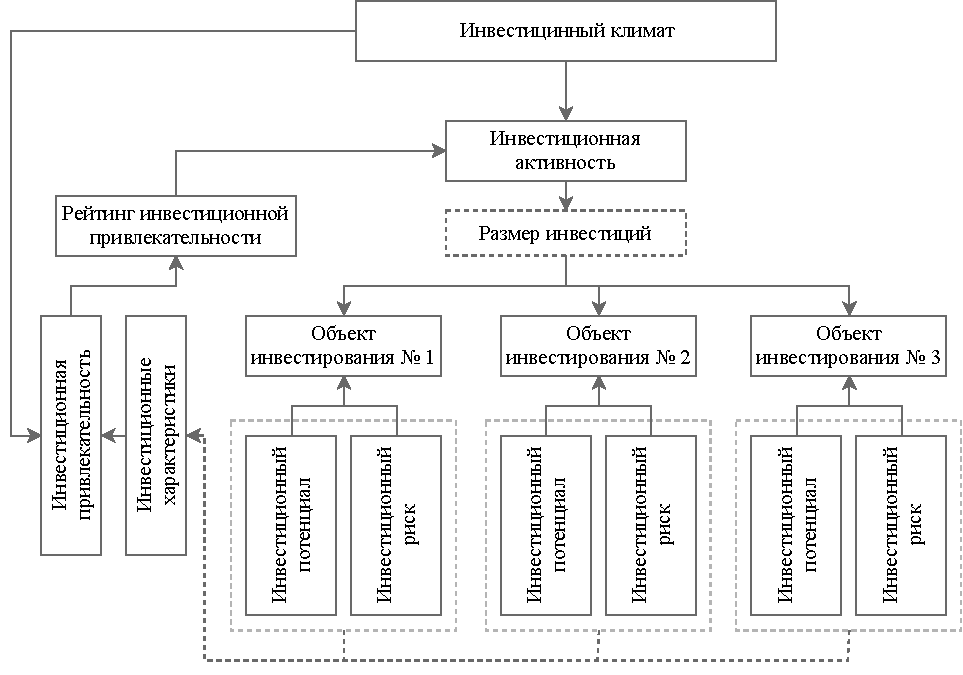
\includegraphics[width=1\linewidth]{invest}
	\caption{Взаимосвязь между инвестиционным климатом, инвестиционной активностью и инвестиционной привлекательностью}
	\label{fig:invest}
\end{figure}

Под инвестиционной активностью понимается динамика размера, структуры инвестиций, а также эффективность их использования.
Она напрямую зависит от рейтингов объектов инвестирования, публикуемых рейтинговыми агентствами и консалтинговыми компаниями.
В настоящее время рассчитываются рейтинги стран, субъектов федерации, городов и организаций.
Ключевое влияние на рейтинг оказывает инвестиционная привлекательность.
Она выражается в наборе качественных характеристик, делающих потенциальный объект  инвестирования безопасным и выгодным вложением для инвесторов.
Рейтинг может быть представлен с помощью индекса, на основе которого сравниваются объекты со схожими качественными характеристиками.

Степень инвестиционной привлекательности объекта зависит от инвестиционного потенциала и инвестиционного риска.
Она определяется совокупностью имеющихся объективных показателей и предпосылок для осуществления инвестиций (инвестиционный потенциал), а также вероятностью возникновения непредвиденных финансовых потерь в условиях неопределенности вложения капитала за счет изменения макроэкономической ситуации (инвестиционный риск).
Степень инвестиционной привлекательности отражается на размере инвестиций в различные объекты.

Российские исследователи выделяют следующие факторы, оказывающие влияние на инвестиционный климат:
\begin{itemize}{\itemsep{0pt}}
	\item политическая стабильность;
	\item нормативно-законодательная база и скорость ее изменения;
	\item состояние внутреннего рынка страны и ее финансовой системы;
	\item размер налогового бремени;
	\item платежеспособный спрос населения;
	\item квалификация персонала;
	\item стоимость ресурсов (сырьевых, трудовых, финансовых);
	\item информационное обеспечение;
	\item задолженность по внешним обязательствам перед международными экономическими и финансовыми организациями.
\end{itemize}

















\subsection{Принципы оценки эффективности инвестиционного проекта}
\subsection{Основные мероприятия, направленные на снижение инвестиционных рисков в проектах}